\documentclass[review,leqno]{siamart1116}
\usepackage{amssymb}
\usepackage{amsmath}
\usepackage{newlfont}
\usepackage{graphicx}
\usepackage{color}  
\usepackage{xspace}
\usepackage{subcaption}
\usepackage{siunitx}
\usepackage{bm}
\usepackage{multirow}
\usepackage{mydef}
\usepackage[numbers]{natbib}
\usepackage{tikz}
\usetikzlibrary{decorations.pathreplacing}
\usetikzlibrary{fadings}
\let\cite=\citet

\newcommand{\eric}[1]{{\color{blue}#1}}
\newcommand{\justin}[1]{{\color{violet}#1}}
\newcommand{\peng}[1]{{\color{cyan}#1}} 

\def\bF{\mathbf F}
\def\bi{\mathbf i}
\def\bj{\mathbf j}
\def\bk{\mathbf k}

\begin{document}

\newcommand\footnotemarkfromtitle[1]{%
\renewcommand{\thefootnote}{\fnsymbol{footnote}}%
\footnotemark[#1]%
\renewcommand{\thefootnote}{\arabic{footnote}}}

% Declare title and authors, without \thanks
\newcommand{\TheTitle}{Using neural nets for identifying divergence free vector fields}

\newcommand{\TheAuthors}{J.Owen, E. Tovar, P. Wei}

% Sets running headers as well as PDF title and authors
\headers{Convolutional neural networks}{\TheAuthors}

% Title.
\title{{\TheTitle}\thanks{Draft version, \today \funding{No funding was given for this project.}}}

% Authors: full names plus addresses.
\author{Justin Owen\footnotemark[3]
%
\and Eric Tovar\footnotemark[3] 
%
\and Peng Wei\footnotemark[3] 
% the names are in alphabetical order
}

\maketitle

\renewcommand{\thefootnote}{\fnsymbol{footnote}} 

%\footnotetext[2]{ERDC.}

\footnotetext[3]{Department of Mathematics, Texas A\&M University 3368
  TAMU, College Station, TX 77843, USA.}

\renewcommand{\thefootnote}{\arabic{footnote}}

\begin{abstract}
  We investigate the use of convolutional neural networks for identifying globally divergence-free vector fields. We show that network architectures used in image classification can be repurposed for identifying globally divergence free vector fields defined on the domain $[-1,1]\times[-1,1]$.
  \end{abstract}

\begin{keywords}
  Neural networks, Deep learning, Convolution Neural Nets, Divergence Free Flows. 
\end{keywords}

\begin{AMS}
62M45, 62M40, 37C10
\end{AMS}

\section{Introduction}
% recall to cite use \cite{}

Machine learning for scientific computing has gained massive attraction 
from researchers across disciplines. 
In \cite{RPK2017a,RPK2017b} a physics informed neural network was constructed 
to tackle data-driven solutions and data-driven discovery of nonlinear 
partial differential equations.
\cite{MST2017} trained a deep convolutional network to predict the ground state energy, kinetic energy, and the first excited-state energy of an electron.


Given a continuously differentiable vector field 
$\bF = u(x,y)\bi + v(x,y)\bj$, 
the divergence of $\bF$ is a scalar-valued function defined by
\[\nabla \cdot \bF = \frac{\partial u}{\partial x} 
+ \frac{\partial v}{\partial y}.\]
We say a vector field is divergence free if $\nabla \cdot \bF = 0$.
In practice, a divergence free vector field implies that the fluid is incompressible. 
Namely, the mass is conserved in $\Omega$ throughout the time. 
Due to such property, the divergence-free vector field is ubiquitous 
in physics, fluid dynamics, geophysics, among others.
To name a few, the magnetic field, the electric field in free space, most familiar liquids, 
and perfect gas are all incompressible. \justin{Given the ubiquity of divergence free vector fields we seek to answer the following question: given a vector field, can a neural net identify if it is divergence free?} We will try to answer the question with the use of convolutional neural nets.

The vector field shares some similarity with the image processing. \eric{Maybe give some more info on the RBG color model? I'm not sure. Or maybe say Red Blue Green (RGC) color model}
In RGB color model, the image is represented by a RGB triplet at each pixel.
In addition, the nearby pixels are more highly correlated than the far away pixels. We consider vector fields defined on a fixed domain \justin{$\Omega:=[-1,1]\times[-1,1] \subset \mathbb{R}^2$ and the domain is discretized into a uniform grid.} The vector field can then be approximately represented by storing a rank 3 tensor,
with two dimensions representing the spatial location, 
and one dimension storing the vector value. Moreover, whenever the vector field is continuous, the values are highly correlated in a small neighbourhood. 
Consequently, there is a hope that by training the neural nets with a similar methodology,
we can come up with a vector field classifier.

This paper is organized as follows.
In section 2, we introduce the families of divergence free and non divergence free vector fields, and use these families of functions as basis to generate our training data set as well as the testing data set.
In section 3, we define our convolutional neural network together with the loss function.
The simulation results are presented in section 4.
We end our paper with conclusions and possible extensions in section 5.

All code and data sets justifying this manuscript can be found at
\url{https://github.com/jowen6/DeepLearningFall2018Project}.

\peng{
Another paper by Brown group:
A deep convolutional neural network for
classification of red blood cells in sickle cell
anemia
\url{https://journals.plos.org/ploscompbiol/article/file?id=10.1371/journal.pcbi.1005746&type=printable}
}


%%%% import files here %%%%%
\section{Data generation}

In this section, we introduce the methods for producing the divergence free and non divergence free vector fields used for training and testing.
\justin{
We know that we can't possibly present every type of divergence free or non divergence free vector field for training. Our hope is that the neural net learns what divergence free means from a small family of divergence free vector fields and is able to properly generalize these ideas. Our setup consists of a set of training data generated from a family of divergence free fields of a specific form. In order to test how well our classifier generalizes we created divergence free vector fields that do not belong to any the family of fields used in training. We refer to these new fields as enrichment sets. Our test data then consists of fields from the families found in the training set as well as fields from the enrichment set.
}


For variety, we consider four families of the divergence free vector fields and two families of non divergence free fields. We give the details of each particular family below and show in \Cref{fig:data_ex} examples of the divergence free fields and in \Cref{fig:data_ex_2} examples of the non divergence free fields.

%%%%%%%%%
\subsection{First family of divergence free vector fields}

\justin{The simplest method of generating a divergence free vector field is to ensure that for a vector \\$\bv = \left(u(x,y),v(x,y)\right)$ we have
$u(x,y) = u(y)$ and $v(x,y)=v(x)$. 
We choose to represent $u(y)$ and $v(x)$ as linear combinations of the basic functions \\$\{x, \cos(2\pi x), \sin(\pi x),e^{x}/e\}$ or}
\begin{align}
    u(y) &= c_1 y + c_2\cos(2\pi y) + c_3 \sin(\pi y) + c_4e^{y}/e,\label{firstClassVX}\\
    v(x) &= d_1 x + d_2\cos(2\pi x) + d_3 \sin(\pi x) + d_4e^{x}/e.\label{firstClassVY}
\end{align}
  
This guarantees that 
 \[ \nabla\cdot \bv = 0.\]

The coefficients corresponding to the vector field functions 
are independent and identically distributed random variables 
drawn from $U(-1,1)$, the uniform distribution in the interval $[-1,1]$.

%%%%%%%
\subsection{Second family of divergence free vector fields}

The second family of divergence free vector fields can be obtained as follows: setting $\bv = \left(f(x,y),g(y)\right)$ initially and choosing $f(x,y)$ simple and smooth, one can find $g(x,y)$ by integrating the simple differential equation with respect to the spatial variable $y$
\[g^{'}(y) = -\frac{\partial f}{\partial x}(x,y). 
\]
Choosing the following functions for $f(x,y)$: $\{c_1 x y^2, c_2 \cos(x) y + c_3 x^2 e^{-y}\}$, we obtain the following family of divergence free fields for $\bv = \left(f(x,y),g(x,y)\right)$

\begin{align}
    f(x,y) &= c_1 x y^2 +  c_2 \cos(x) y + c_3 x^2 e^{-y},\label{secondClassVX}\\
    g(x,y) &= -c_1\frac{y^3}{3} + c_2 \frac{1}{2}y^2\sin(x) + 2c_3xe^{-y},\label{secondClassVY}
\end{align}
where $c_1,c_2,c_3\in U(-1,1)$.
%%%%%%%
\subsection{Third family of divergence free vector fields}
For this next family, we consider a \textit{high frequency} type of divergence free vector field. That is, we set the components of our vector $\bv$ to be highly oscillatory trigonometric functions: 
\begin{align}
    u(y) &= \sin(32\pi y),\label{thirdClassVX}\\
    v(x) &= \cos(32\pi x).\label{thirdClassVY}
\end{align}
\justin{We choose this because our grid sampling only has 64 points and this is the Nyquist frequency. In other words, the 32 Hz is the upper limit on frequencies that our grid can resolve.}
%%%%%%%
\subsection{Fourth family of divergence free vector fields}
For this next family, we consider a \textit{low frequency} type of divergence free vector field. That is, we set the components of our vector $\bv$ to be low oscillatory trigonometric functions: 
\begin{align}
    u(y) &= \sin(\frac{1}{32}\pi y),\label{fourthClassVX}\\
    v(x) &= \cos(\frac{1}{32}\pi x).\label{fourthClassVY}
\end{align}
We choose this particular family because on the computational domain $[-1,1] \times [-1,1]$ the field is very close to being flat. We wanted to test how the neural network performed with an \textit{extreme} case. 

%%%%%%% all families of divergence free figure %%%%%%%
\begin{figure}[ht]
		\begin{center}
			\begin{tabular}{cc}
				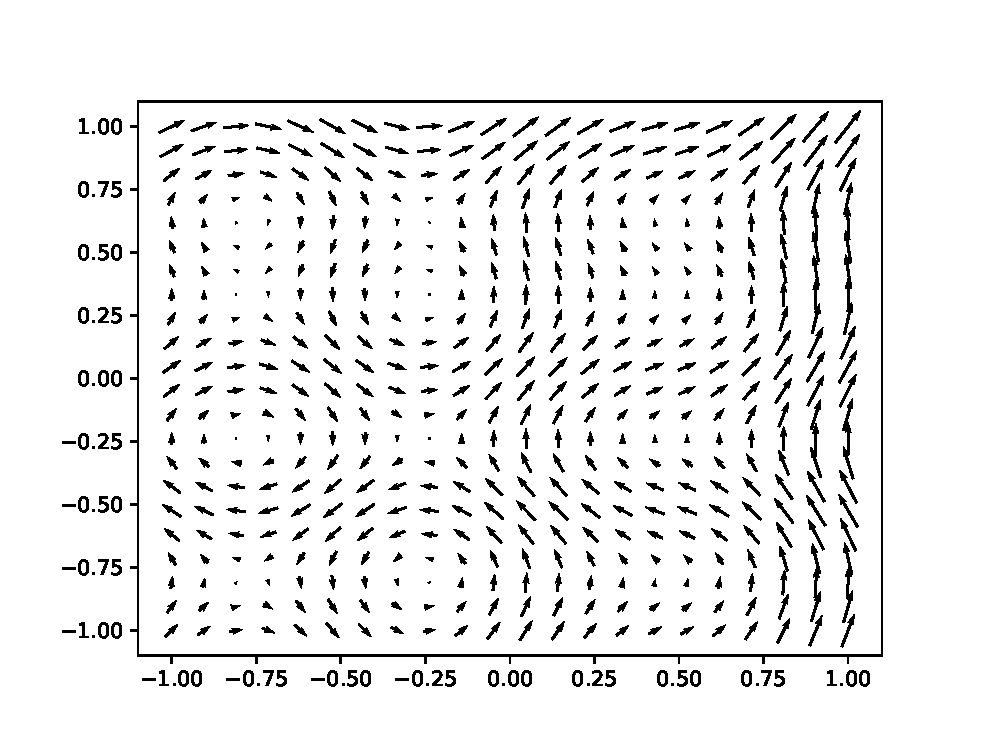
\includegraphics[scale=.40]{first_div_field.eps}&
				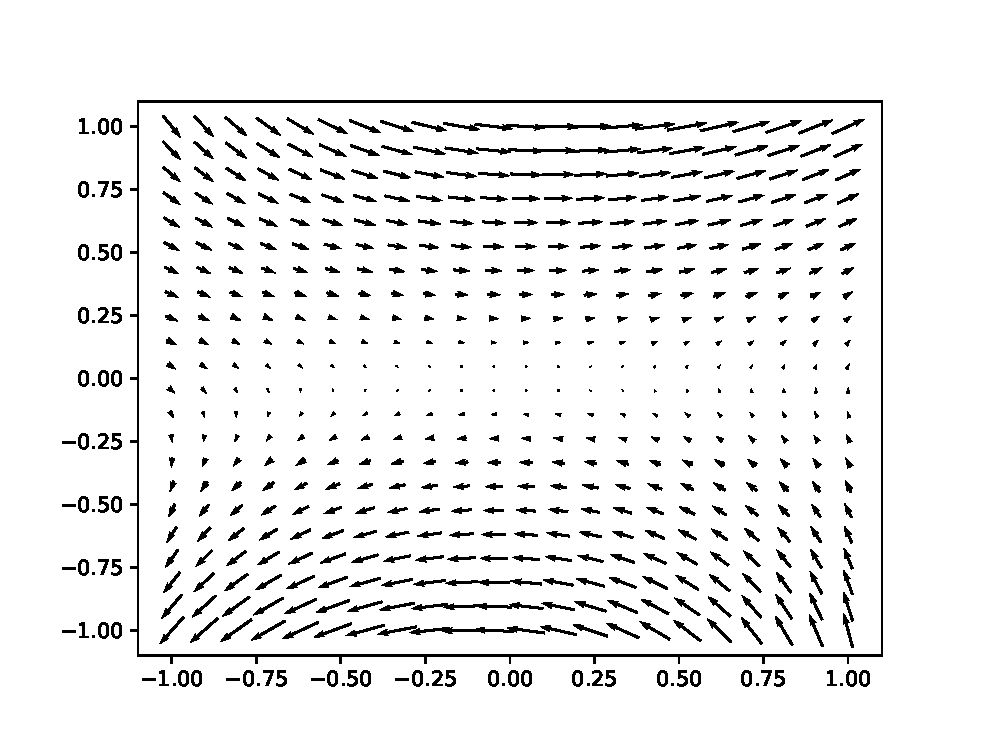
\includegraphics[scale=.40]{second_div_field.eps} \\
				(a) & (b)\\
				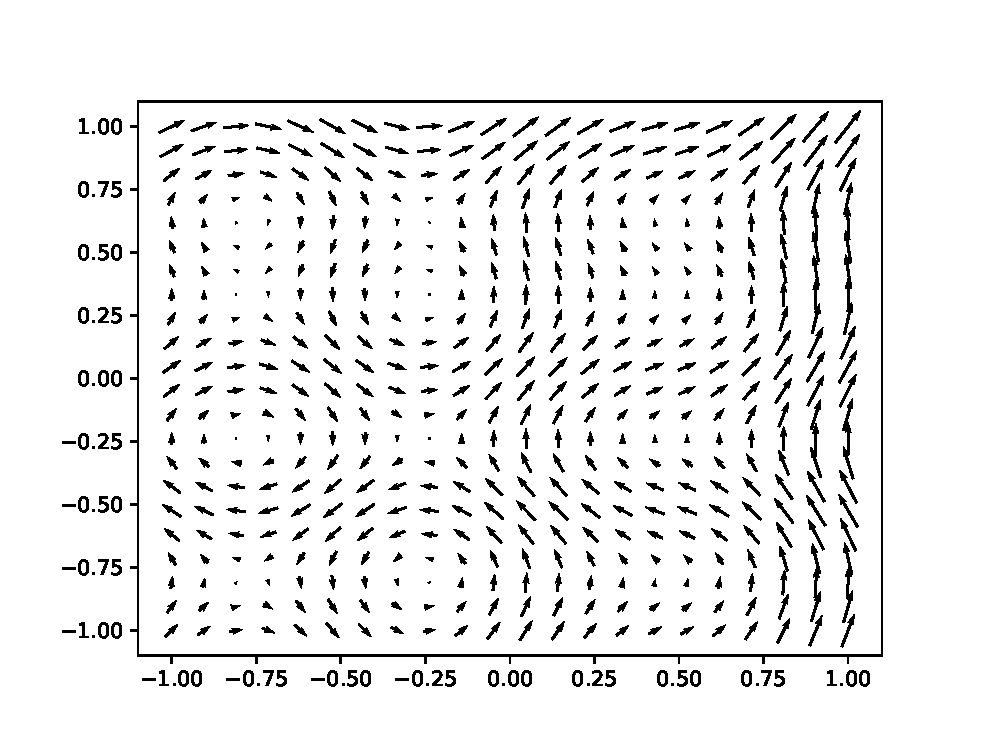
\includegraphics[scale=.40]{first_div_field.eps}&
				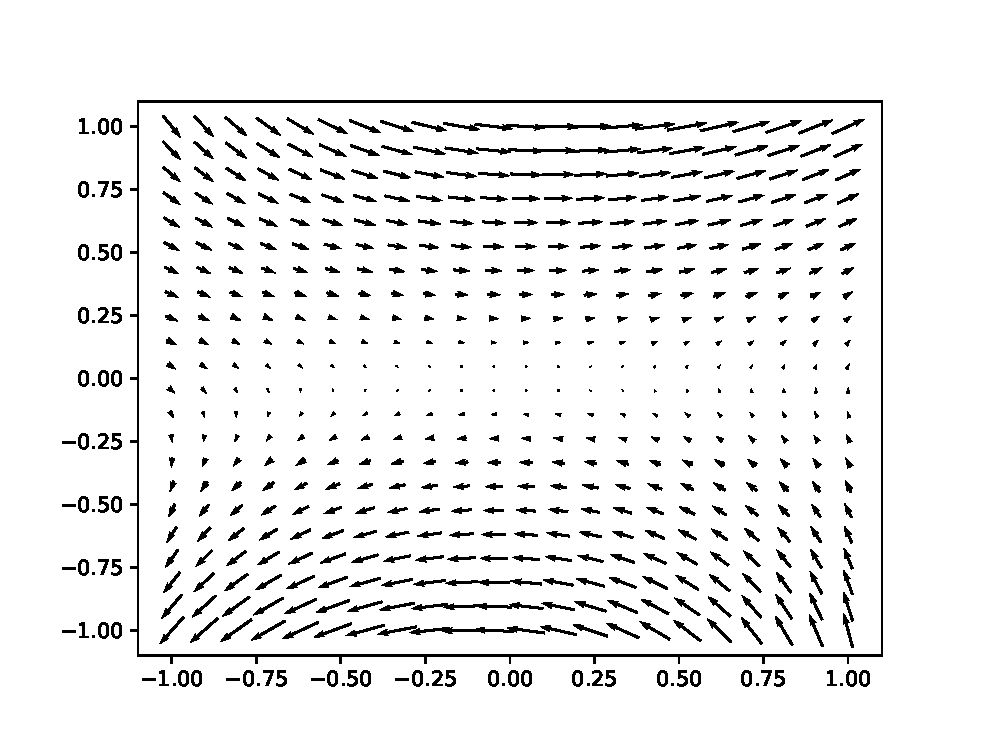
\includegraphics[scale=.40]{second_div_field.eps} \\
				(c) & (d)
			\end{tabular}
		\end{center}
		\caption{Examples of divergence free generated vector fields.
			(a). First class; 
			(b). Second class;
			(c). Third class;
			(d). Fourth class.
			}
		\label{fig:data_ex}
\end{figure}
%%%%%%%%%% end figure %%%%%%%%%%%%%
\section{Convolutional neural net}
\peng{
Given two functions $f,g:\{-n, \cdots, n\}\to \polR$, the discrete convolution is defined by
\[(f*g)(x) = \sum_{y = -n}^{n} f(y)g(x-y).\]
The ReLU net is defined by
\[ ReLU(t) = \max{0,t}.\]
The convolutional neural networks, denoted by ConvNets, consist of three different types of layers:
convolutional layer, pooling layer, and fully connected layer.
The architecture is of this form:
\[
\textrm{Input} \to 
\underbrace{[\textrm{Conv} \to \textrm{ReLU} \to \textrm{Pool]}}
_\textrm{N times} 
\to \textrm{FC}
\]
\textbf{PW: Need descriptions of the CONV, ReLU Pool and FC layers. 
Resource: \url{http://cs231n.github.io/convolutional-networks/}}

After applying the fully-connected layer, we obtain a vector of scores 
$\mathbf v(x) = (v_1(x), \cdots v_n(x))$. 
We first apply the soft-max
\[ (\mu_1(x),\cdots, \mu_n(x)) 
= SM(x) = \left( \frac{e^{v_1}}{\sum_i e^{v_i}}, 
\cdots  \frac{e^{v_n}}{\sum_i e^{v_i}}  \right). \]
The cross entropy loss function is defined as
\[\mathcal L (x) = -\sum_{j = 1}^n \log(\frac{e^{v_j}}{\sum_i e^{v_i}}).  \]

}
\begin{figure}[t!]
	\centering
	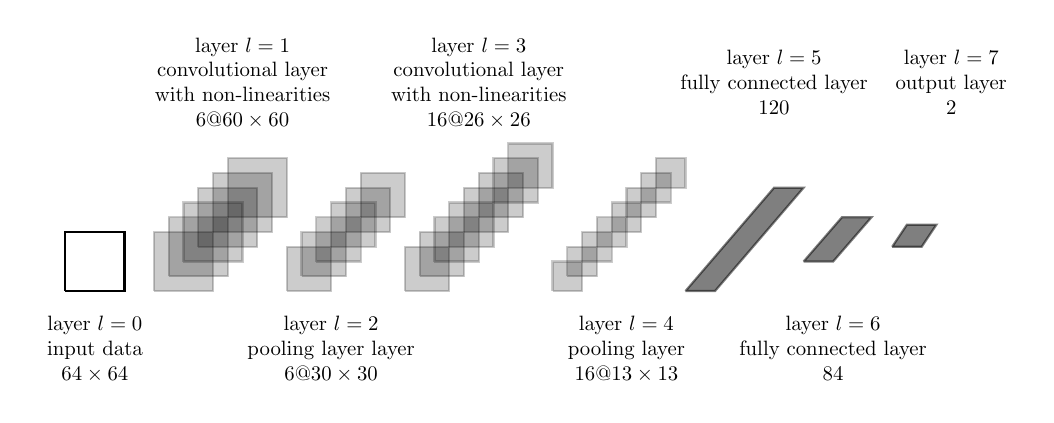
\begin{tikzpicture}[thick,scale=0.75, every node/.style={scale=0.75}]
		\node at (0.5,-1){\begin{tabular}{c}layer $l = 0$\\input data\\ $64\times 64$ \end{tabular}};
		
		\draw (0,0) -- (1,0) -- (1,1) -- (0,1) -- (0,0);
		
		\node at (3,3.5){\begin{tabular}{c}layer $l = 1$\\convolutional layer\\with non-linearities\\$6@60\times 60$\end{tabular}};
		
		\draw[fill=black,opacity=0.2,draw=black] (2.75,1.25) -- (3.75,1.25) -- (3.75,2.25) -- (2.75,2.25) -- (2.75,1.25);
		\draw[fill=black,opacity=0.2,draw=black] (2.5,1) -- (3.5,1) -- (3.5,2) -- (2.5,2) -- (2.5,1);
		\draw[fill=black,opacity=0.2,draw=black] (2.25,0.75) -- (3.25,0.75) -- (3.25,1.75) -- (2.25,1.75) -- (2.25,0.75);
		\draw[fill=black,opacity=0.2,draw=black] (2,0.5) -- (3,0.5) -- (3,1.5) -- (2,1.5) -- (2,0.5);
		\draw[fill=black,opacity=0.2,draw=black] (1.75,0.25) -- (2.75,0.25) -- (2.75,1.25) -- (1.75,1.25) -- (1.75,0.25);
		\draw[fill=black,opacity=0.2,draw=black] (1.5,0) -- (2.5,0) -- (2.5,1) -- (1.5,1) -- (1.5,0);
		
		\node at (4.5,-1){\begin{tabular}{c}layer $l = 2$\\pooling layer layer\\$6@30\times30$\end{tabular}};
		
		\draw[fill=black,opacity=0.2,draw=black] (5,1.25) -- (5.75,1.25) -- (5.75,2) -- (5,2) -- (5,1.25);
		\draw[fill=black,opacity=0.2,draw=black] (4.75,1) -- (5.5,1) -- (5.5,1.75) -- (4.75,1.75) -- (4.75,1);
		\draw[fill=black,opacity=0.2,draw=black] (4.5,0.75) -- (5.25,0.75) -- (5.25,1.5) -- (4.5,1.5) -- (4.5,0.75);
		\draw[fill=black,opacity=0.2,draw=black] (4.25,0.5) -- (5,0.5) -- (5,1.25) -- (4.25,1.25) -- (4.25,0.5);
		\draw[fill=black,opacity=0.2,draw=black] (4,0.25) -- (4.75,0.25) -- (4.75,1) -- (4,1) -- (4,0.25);
		\draw[fill=black,opacity=0.2,draw=black] (3.75,0) -- (4.5,0) -- (4.5,0.75) -- (3.75,0.75) -- (3.75,0);
		
		\node at (7,3.5){\begin{tabular}{c}layer $l = 3$\\convolutional layer\\with non-linearities\\$16@26\times26$\end{tabular}};
		
		\draw[fill=black,opacity=0.2,draw=black] (7.5,1.75) -- (8.25,1.75) -- (8.25,2.5) -- (7.5,2.5) -- (7.5,1.75);
		\draw[fill=black,opacity=0.2,draw=black] (7.25,1.5) -- (8,1.5) -- (8,2.25) -- (7.25,2.25) -- (7.25,1.5);
		\draw[fill=black,opacity=0.2,draw=black] (7,1.25) -- (7.75,1.25) -- (7.75,2) -- (7,2) -- (7,1.25);
		\draw[fill=black,opacity=0.2,draw=black] (6.75,1) -- (7.5,1) -- (7.5,1.75) -- (6.75,1.75) -- (6.75,1);
		\draw[fill=black,opacity=0.2,draw=black] (6.5,0.75) -- (7.25,0.75) -- (7.25,1.5) -- (6.5,1.5) -- (6.5,0.75);
		\draw[fill=black,opacity=0.2,draw=black] (6.25,0.5) -- (7,0.5) -- (7,1.25) -- (6.25,1.25) -- (6.25,0.5);
		\draw[fill=black,opacity=0.2,draw=black] (6,0.25) -- (6.75,0.25) -- (6.75,1) -- (6,1) -- (6,0.25);
		\draw[fill=black,opacity=0.2,draw=black] (5.75,0) -- (6.5,0) -- (6.5,0.75) -- (5.75,0.75) -- (5.75,0);
		
		\node at (9.5,-1){\begin{tabular}{c}layer $l = 4$\\pooling layer\\$16@13\times13$\end{tabular}};
		
		\draw[fill=black,opacity=0.2,draw=black] (10,1.75) -- (10.5,1.75) -- (10.5,2.25) -- (10,2.25) -- (10,1.75);
		\draw[fill=black,opacity=0.2,draw=black] (9.75,1.5) -- (10.25,1.5) -- (10.25,2) -- (9.75,2) -- (9.75,1.5);
		\draw[fill=black,opacity=0.2,draw=black] (9.5,1.25) -- (10,1.25) -- (10,1.75) -- (9.5,1.75) -- (9.5,1.25);
		\draw[fill=black,opacity=0.2,draw=black] (9.25,1) -- (9.75,1) -- (9.75,1.5) -- (9.25,1.5) -- (9.25,1);
		\draw[fill=black,opacity=0.2,draw=black] (9,0.75) -- (9.5,0.75) -- (9.5,1.25) -- (9,1.25) -- (9,0.75);
		\draw[fill=black,opacity=0.2,draw=black] (8.75,0.5) -- (9.25,0.5) -- (9.25,1) -- (8.75,1) -- (8.75,0.5);
		\draw[fill=black,opacity=0.2,draw=black] (8.5,0.25) -- (9,0.25) -- (9,0.75) -- (8.5,0.75) -- (8.5,0.25);
		\draw[fill=black,opacity=0.2,draw=black] (8.25,0) -- (8.75,0) -- (8.75,0.5) -- (8.25,0.5) -- (8.25,0);
		
		\node at (12,3.5){\begin{tabular}{c}layer $l = 5$\\fully connected layer\\ $120$\end{tabular}};
		
		\draw[fill=black,draw=black,opacity=0.5] (10.5,0) -- (11,0) -- (12.5,1.75) -- (12,1.75) -- (10.5,0);
		
		\node at (13,-1){\begin{tabular}{c}layer $l = 6$\\fully connected layer\\$84$\end{tabular}};
		
		\draw[fill=black,draw=black,opacity=0.5] (12.5,0.5) -- (13,0.5) -- (13.65,1.25) -- (13.15,1.25) -- (12.5,0.5);
		
		\node at (15,3.5){\begin{tabular}{c} layer $l = 7$\\output layer\\$2$\end{tabular}};
		
		\draw[fill=black,draw=black,opacity=0.5] (14,0.75) -- (14.5,0.75) -- (14.75,1.125) -- (14.25,1.125) -- (14,0.75);
		
	\end{tikzpicture}
	\caption[Architecture of our convolutional neural network.]
	{The architecture of our convolutional neural network. 
	The convolutional layers (layers 1 and 3) actually represent two layers, with the ReLU net hidden, thus they already include non-linearities. 
	The output layer uses softmax activation functions.}
	\label{fig:traditional-convolutional-network}
\end{figure}



\section{Results}
\peng{
Here are some turning parameters that I can think of:
\begin{itemize}
    \item Training data size $M$,
    \item The ratio $\alpha$ of divergence free data sets in $M$, 
    \item The learning rate $\lambda$,
    \item The ConvNet structure.
\end{itemize}


}

\justin{
Some issues we may wish to present:
\begin{itemize}
    \item The success rate on the entire test set for cases of enriched and not enriched test data.
    \item How well the softmax scores distinguish between div and non div. Discuss how the training set size doesn't appear in the success rate, but does have a major effect on how well the softmax scores separate.
    \item Even though the accuracy of our classifier is quite high on the overall test set, we wanted to know how the score the neural net gave for individual vector fields changed as a function of the training data. One could think of this as how confident the network becomes in its classifications as it is trained with more data. In figure BLAH we have 
    
\end{itemize}


\begin{figure}[ht]
		\begin{center}
			\begin{tabular}{cc}
				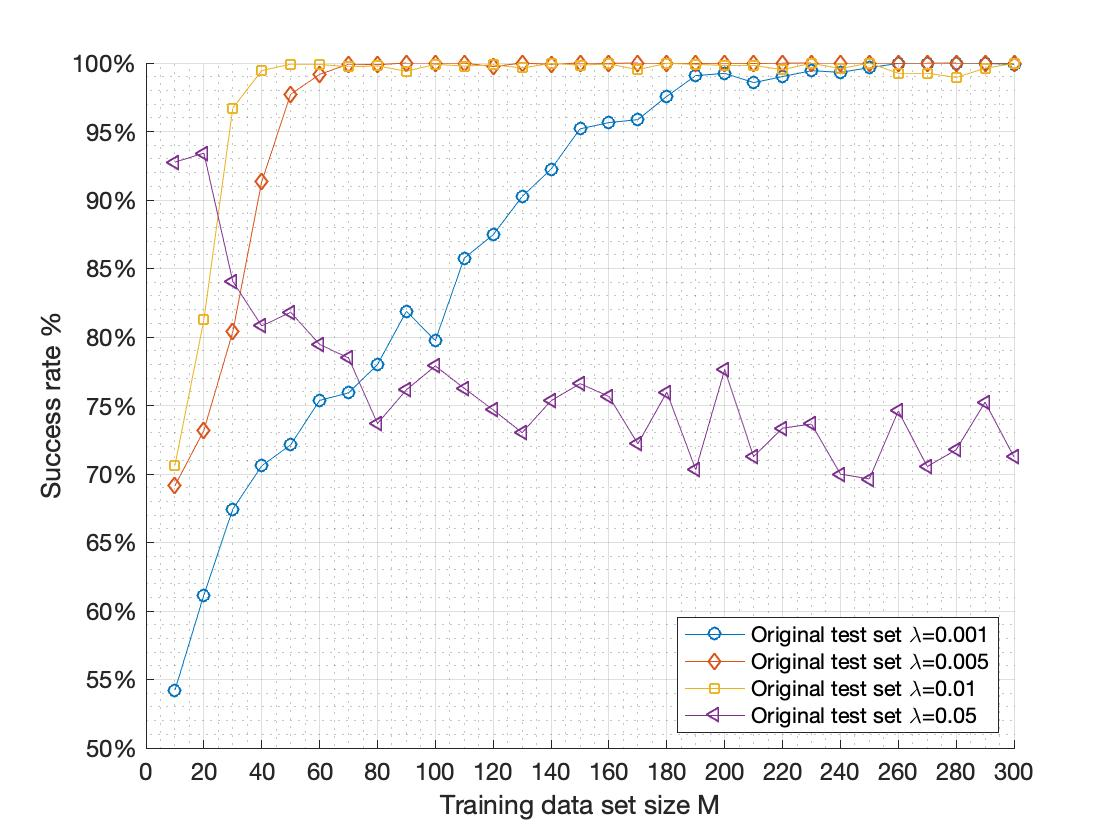
\includegraphics[scale=.15]{orig_sr.jpg}&
				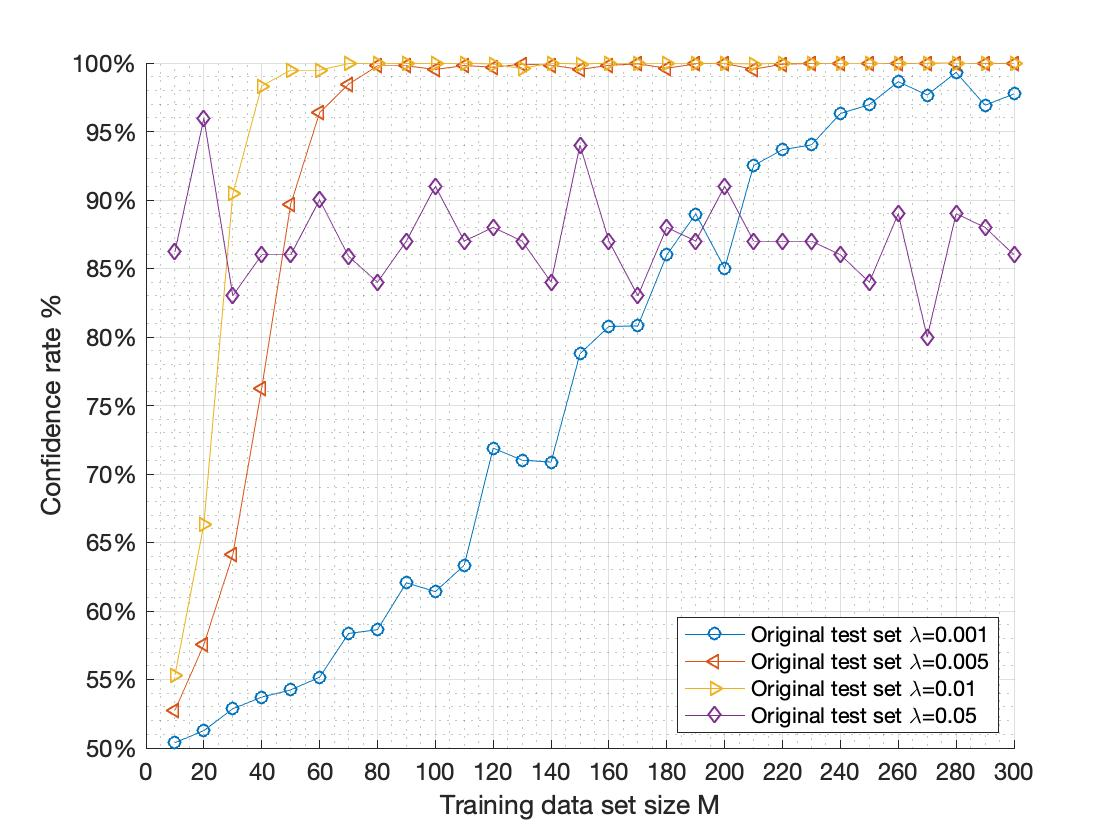
\includegraphics[scale=.15]{orig_cr.jpg} \\
				(a) & (b)
			\end{tabular}
		\end{center}
		\caption{Testing results on original set. 
		(a) The success rate
		(b) The confidence rate on identifying a specific vector field.
		}
		\label{fig:orig_results}
\end{figure}

}
\section{Conclusion and future work}
Conclusion goes here

\eric{Since we are now only testing on a subset of divergence free vector fields, our hope is to be able to test on any random vector field and be able to tell how close the field is close to being divergence free. We think we can further extend this to being able to identify local areas of the divergence free   }
%%%% import files here %%%%%

\bibliographystyle{abbrvnat} 
\bibliography{ref}

\end{document}

%%% Local Variables:
%%% mode: latex
%%% mode: flyspell
%%% TeX-master: t
%%% End: 